\documentclass[11pt, answers]{exam}
\usepackage[utf8]{inputenc}
\usepackage[T1]{fontenc}
\usepackage{amsmath, amssymb, amsopn, color, tikz, mathtools}
\usepackage[margin=1in]{geometry}
\usepackage{titlesec}
\usepackage{tipa}
\usepackage{hyperref}


% Style
\setlength\parindent{0pt}
\shadedsolutions

% Define course info
\def\semester{Semestre 2}
\def\course{Modèle de duréee M1 DUAS}
\def\name{P.-O. Goffard}
%\def\quizdate{10/5, 10/6}
\def\hwknum{}
%\def\title{\MakeUppercase{Homework \hwknum -- quiz \quizdate }}
\def\title{\MakeUppercase{TD 1: Approche paramétrique de la survie.}}
% Distributions.
\newcommand*{\UnifDist}{\mathsf{Unif}}
\newcommand*{\ExpDist}{\mathsf{Exp}}
\newcommand*{\DepExpDist}{\mathsf{DepExp}}
\newcommand*{\GammaDist}{\mathsf{Gamma}}
\newcommand*{\LognormalDist}{\mathsf{LogNorm}}
\newcommand*{\WeibullDist}{\mathsf{Weib}}
\newcommand*{\ParetoDist}{\mathsf{Par}}
\newcommand*{\NormalDist}{\mathsf{Normal}}

\newcommand*{\GeometricDist}{\mathsf{Geom}}
\newcommand*{\NegBinomialDist}{\mathsf{NegBin}}
\newcommand*{\BinomialDist}{\mathsf{Bin}}
\newcommand*{\PoissonDist}{\mathsf{Poisson}}

% Sets of numbers.
\newcommand*{\RL}{\mathbb{R}}
\newcommand*{\N}{\mathbb{N}}
\newcommand*{\NZ}{\mathbb{N}_0}
% \newcommand*{\NL}{\mathbb{N}_+}

\newcommand*{\cond}{\mid}
\newcommand*{\given}{\,;\,}

%Probability symbols
\newcommand*{\Prob}{\mathbb{P}}
\newcommand*{\Q}{\mathbb{Q}}
\newcommand*{\E}{\mathbb{E}}
\newcommand*{\F}{\mathcal{F}}
% Regarding spacing and abbreviations.
\usepackage{xspace}

% Acronyms
% \@\xspace doesn't add space if next char is punctuation
% However, these will give 2 .'s if used at end of sentence.
\newcommand*{\eg}{e.g.\@\xspace}
\newcommand*{\ps}{p.s.\@\xspace}
\newcommand*{\ie}{i.e.\@\xspace}
\newcommand*{\va}{v.a.\@\xspace}
\newcommand*{\iid}{i.i.d.\@\xspace}
\newcommand*{\ssi}{s.s.i.\@\xspace}
\newcommand*{\cf}{c.f.\@\xspace}
\newcommand*{\pdf}{p.d.f.\@\xspace}
\newcommand*{\pmf}{p.m.f.\@\xspace}
\newcommand*{\cdf}{c.d.f.\@\xspace}
\newcommand*{\SMC}{\textbf{SMC}\@\xspace}
\newcommand*{\MCMC}{\textbf{MCMC}\@\xspace}
\newcommand*{\VF}{\textbf{VF}\@\xspace}


\newcommand*{\iidSim}{\overset{\mathrm{i.i.d.}}{\sim}}
\newcommand*{\bt}{\bm{\theta}}
\newcommand*{\bTheta}{\bm{\Theta}}
\newcommand*{\bbeta}{\bm{\beta}}
\newcommand*{\bx}{\mathbf{x}}
\newcommand*{\bs}{\bm{s}}
\newcommand*{\bu}{\bm{u}}
\newcommand*{\bn}{\bm{n}}

% Roman versions of things.
\newcommand*{\dd}{\mathop{}\!\mathrm{d}}
\newcommand*{\e}{\mathrm{e}}
\DeclareMathOperator*{\argmax}{arg\,max}
\DeclareMathOperator*{\argmin}{arg\,min}

\newcommand*{\norm}[1]{\lVert{} #1\rVert}

% \DeclarePairedDelimiterXPP{\ind}[1]{\ind_}{\{}{\}}{}{#1}
\newcommand*{\ind}{\mathbb{I}}
\def\euro{\mbox{\raisebox{.25ex}{{\it =}}\hspace{-.5em}{\sf C}}}
  \everymath{\displaystyle}
% \newcommand{\limsup}{\overline{\lim}\,}            % blackboard P
% \newcommand{\liminf}{\underline{\lim}\,}            % blackboard P

\begin{document}

% Heading
{\center \textsc{\Large\title}\\
	\vspace*{1em}
	\course -- \semester\\
	\name\\
	\vspace*{2em}
	\hrule
\vspace*{2em}}

\begin{questions}
\question L'objectif est de déterminer l'estimateur du maximum de vraisemblance de la loi exponentielle $\ExpDist(\beta)$ de densité 
$$
f(t) = \frac{\e^{-t/\beta}}{\beta}\ind_{(0,\infty)}(t).
$$
Soit $\mathcal{D} = \{t_1, \ldots,t_n\}$ un échantillon \iid de réalisations d'une \va exponentielle.
\begin{parts}
\part Donner l'estimateur du maximum de vraisemblance $\widehat{\beta}$.
\begin{solution}
La log vraisemblance s'écrit
$$
l(\mathcal{D};\beta) = -n\log(\beta)-\frac{1}{\beta}\sum t_i.
$$
On a 
$$
\frac{\partial l}{\partial \beta}(\mathcal{D};\beta) = -n\frac{n}{\beta}+\frac{1}{\beta^2}\sum t_i.
$$
On en déduit que 
$$
\frac{\partial l}{\partial \beta}(\mathcal{D};\beta) = 0\Leftrightarrow \widehat{\beta} = \frac{\sum t_i}{n},
$$
après avoir vérifié que
$$
\frac{\partial l}{\partial \beta}(\mathcal{D};\widehat{\beta}) < 0.
$$
\end{solution}
\part Supposons que nous soyons en présence de données censurées, avec une censure à droite, non informative, de niveaux $c_1,\ldots, c_n$. Donner l'estimateur du maximum de vraisemblance de $\beta$.

\begin{solution}
Les observations sont 
$$
(x_i,\delta_i) = (t_i\land c_i, \mathbb{I}_{t_i\leq c_i}),
$$
et la log vraisemblance s'écrit
$$
-\sum \delta_i\log(\beta)-\frac{\sum x_i}{\beta} + \text{Cste}.
$$
On en déduit que
$$
\frac{\partial l}{\partial \beta}(\mathcal{D};\beta) = 0\Leftrightarrow \widehat{\beta} = \frac{\sum x_i}{\sum \delta_i}.
$$
On peut vérifier la cohérence de l'estimation. En prenant $C\rightarrow \infty$, on retombe sur l'estimateur obtenu à la question 1.
\end{solution}

% \part Supposons que nous soyons en présence de données censurées, avec une censure de type II avec arrêt au $r^{\text{ème}}$ évènement et $r\leq n$. Donner l'estimateur du maximum de vraisemblance de $\beta$.
% \begin{solution}
% En cas de censure de type II, les observations sont 
% $$
% (x_i,\delta_i) = (t_i\land t_{(r)}, \mathbb{I}_{t_i\leq t_{(r)}}),
% $$
% L'estimateur est exactement le même qu'à la question 2.
% \end{solution}

% \part Supposons que nous soyons en présence de données censurées, avec une censure de type de niveau $c_1,\ldots, c_n$. Donner l'estimateur du maximum de vraisemblance de $\beta$.
% \begin{solution}
% En cas de censure de type III, les observations sont 
% $$
% (x_i,\delta_i) = (t_i\land c_i, \mathbb{I}_{t_i\leq c_i}),
% $$
% L'estimateur est exactement le même qu'à la question 2.
% \end{solution}
\part Supposons que nous soyons en présence de données tronquées, avec une troncature à gauche, non informative, de niveaux $c$ pour $i = 1,\ldots, n$. Donner l'estimateur du maximum de vraisemblance de $\beta$.

\begin{solution}
La densité de probabilité pour des observation tronquées à gauche au niveau $c$ est donnée par 
$$
f_{[c,\infty)]}(t) = \frac{\e^{-\beta t}}{\beta\e^{-\beta c}}\mathbb{I}_{[c,\infty)]}(t).
$$
La log-vraisemblance s'écrit 
$$
l(\mathcal{D};\beta) = -n\ln(\beta)-\left[\sum_i t_i - nc\right] /\beta.
$$
On en déduit que
$$
\frac{\partial l}{\partial \beta}(\mathcal{D};\beta) = 0\Leftrightarrow \widehat{\beta} = \frac{\sum x_i}{n} - c.
$$
On peut vérifier la cohérence de l'estimation. En prenant $c = 0$, on retombe sur l'estimateur obtenu à la question 1.
\end{solution}
\end{parts}
\question Soit $T$ la durée d'un évènement, la durée de vie résiduelle $X$ d'un évènement ayant commencé il y a $\theta$ unités de temps est définie par 
$$
X_\theta \sim  T-\theta|T>\theta.
$$
Il s'agit par exemple de la durée de vie résiduelle d'un individu d'âge $\theta$. On notera $S_\theta(x) = \Prob(X_\theta>x)$
\begin{parts}
\part Exprimer l'espérance de vie $\E(T)$ en fonction d'une intégrale de $S(t) = \mathbb{P}(T>t)$
\begin{solution}
On ré-écrit la v.a. $T$ comme 
$$
T = \int_0^{\infty}\mathbb{I}_{[0,T]}(t)\text{d}t
$$
puis par définition de l'espérance et le théorème de Fubini-Tonnelli, il vient
\begin{eqnarray*}
\E(T) &=& \int_\Omega \int_0^{\infty}\mathbb{I}_{[0,T]}(t)\text{d}t\text{d}\Prob\\
&=&  \int_0^{\infty}\int_\Omega\mathbb{I}_{[0,T]}(t)\text{d}\Prob\text{d}t\\
&=&  \int_0^{\infty}S(t)\text{d}t.
\end{eqnarray*}
\end{solution}
\part Exprimer la fonction de durée de vie résiduelle $\E(X_\theta):= \E(X-\theta|X >\theta)$ en fonction d'une intégrale de $S(t)$.
\begin{solution}
On peut commencer par donner la fonction de survie de $X_\theta$ en fonction de $T$, il vient 
$$
S_\theta(x) = \Prob(X - \theta >x|X>\theta) =  \Prob(X >x +\theta|X>\theta) = \frac{S(x+\theta)}{S(\theta)}.
$$
On utilise ensuite la question précédente pour écrire 
$$
\mathbb{E}(X_\theta) = \int_0^\infty\frac{S(x+\theta)}{S(\theta)}\text{d}x.
$$
\end{solution}
\part A partir de maintenant, nous supposons que $X_\theta \sim \ParetoDist(\alpha, \theta)$ (loi de Pareto), avec $\alpha >1$ tel que 
$$
S_\theta(x)  =\theta^\alpha(x+\theta)^{- \alpha},\text{ }x>0.
$$
Calculer $\E(X_\theta)$. Pensez-vous que ce modèle est adapté à la durée de vie humaine? 
\begin{solution}
\begin{equation*}
\E(X_\theta) = \int_0^\infty S_\theta(x)\text{dx} = \frac{\theta}{\alpha-1}.
\end{equation*}
Ce modèle n'est pas adapté car la durée de vie résiduelle augmente avec l'âge !
\end{solution}
\part Soit un évènement ayant duré $\theta$ unités de temps, exprimer la fonction de survie $S_{Y_x}(t)$ de 
$$
Y_x \sim X_\theta - x|X_\theta >x
$$
il s'agit de la durée résiduelle dans $x$ unités de temps d'un évènement ayant déjà durée $\theta$ unités de temps. Quelle remarque peut-on faire?
\begin{solution}
Soit $0< x < y$, on a 
$$
S_{Y_x}(y) = \frac{S_{\theta} (y+x)}{S_{\theta} (x)} = \left(\frac{\theta+ x}{\theta +y}\right)^\alpha = \left(\frac{\theta+ x}{\theta +x + y}\right)^\alpha.
$$
On observe que la durée de vie résiduelle pour une loi de Pareto est encore distribué suivant une loi de Pareto puisque 
$$
Y_x\sim\ParetoDist(\alpha,\theta+x).
$$
\end{solution}
\part Soit un groupe de $n$ évènements ayant déja durés $\theta_1,\ldots, \theta_n$ unités de temps respectivement. Nous observons les durées de vie résiduelles suivantes $\mathcal{D} = \{x_1,\ldots, x_n\}$, donner l'estimateur du maximum de vraisemblance de $\alpha$. 
\begin{solution}
La fonction de vraisemblance s'écrit
$$
L(\mathcal{D};\alpha)  =\prod_{i=1}^{n}f_{\theta_i}(x_i),
$$                                                             
où 
$$
f_\theta(x) = -S_{\theta}'(x) = \alpha\theta^\alpha(x+\theta)^{-\alpha-1}.
$$                   
La log-vraisemblance s'écrit donc 
$$
l(\mathcal{D};\alpha) = \alpha \sum_{i = 1}^n\log(\theta_i)+ n\log(\alpha)-(\alpha + 1)\sum_{i = 1}^n\log(\theta_i + x_i)
$$
L'estimateur du maximum de vraisemblance est donnée par 
$$
\widehat{\alpha} = \frac{n}{\sum_{i=1}^n\log\left(1+\frac{\theta_i}{x_i}\right)}.
$$

\end{solution}
\part Supposons que notre groupe d'évènement n'est observé que pendant $c$ années. Donner l'estimateur du maximum de vraisemblance de $\alpha$ pour les données censurées à droite avec 
$$
z_i = x_i\land c,\text{ }i = 1,\ldots, n.
$$
\begin{solution}
On note $\delta_i = \mathbb{I}_{x_i < c}$ et $\mathcal{D} = \{(z_i,\delta_i)\}_{i =1,\ldots, n}$. La fonction de vraisemblance s'écrit 
$$
L(\mathcal{D};\alpha) = \prod_{i=1}^nh_{\theta_i}(z_i)^{\delta_i}S_{\theta_i}(z_i),
$$
où 
$$
h_\theta(x) = \frac{f_\theta(x)}{S_{\theta}(x)} = \frac{\alpha}{x+\theta}.
$$
On en déduit la log-vraisemblance avec
$$
l(\mathcal{D};\alpha) = \log(\alpha)\sum_{i=1}^n\delta_i-\sum_{i=1}^n \delta_i\log(z_i+\theta_i) + \alpha\sum_{i=1}^n\log(\theta_i) -  \alpha\sum_{i=1}^n\log(\theta_i + z_i).
$$
L'estimateur du maximum de vraisemblance est donné par 
$$
\widehat{\alpha} = \frac{\sum_i \delta_i}{\log\left(1 + \frac{\theta_i}{z_i}\right)}
$$
\end{solution}
\end{parts}
\question Nous allons construire un test d'adéquation à la loi exponentielle $\ExpDist(\beta)$ de densité 
$$
f(t) = \frac{\e^{-t/\beta}}{\beta}\ind_{(0,\infty)}(t),
$$
basé sur la transformée de Laplace. La transformée de Laplace d'une \va $T$ est donnée par 
$$
\psi(\theta) = \mathbb{E}(\e^{-\theta T}).
$$
\begin{parts}
\part Soit $t_1, \ldots, t_n$ un échantillon \iid de réalisation de $T\sim \ExpDist(\beta)$. L'estimateur du maximum de vraisemblance de $\beta$ est donnée par 
$$
\widehat{\beta}_n = \frac{1}{n}\sum_{i=1}^n t_i.
$$
Quelle est la distribution de $T/\widehat{\beta}_n$ lorsque $n\rightarrow\infty$?
\begin{solution}
$T/\widehat{\beta}_n\overset{D}{\rightarrow} \ExpDist(1)$, il s'agit d'une application du théorème de Slutsky \url{https://en.wikipedia.org/wiki/Slutsky%27s_theorem}.
\end{solution}
\part Donner l'expression de la transformée de Laplace $\psi(\theta) = \E(e^{-\theta Y})$ de $Y\sim \ExpDist(\beta=1)$ et montrer qu'elle vérifie l'équation différentielle suivante
$$
\psi'(\theta)(1+\theta) + \psi(\theta) = 0
$$
\begin{solution}
On a
$$
\psi(\theta) = \frac{1}{1+\theta}
$$
et 
$$
\psi'(\theta) = -\frac{1}{(1+\theta)^2} =- \frac{1}{1+\theta}\psi(\theta)
$$
\end{solution}
\part On définit $y_i = t_i/\widehat{\beta}_n$ et
$$
\psi_n(\theta)=\frac{1}{n}\sum_{i=1}^ne^{-\theta y_i}
$$
A quoi correspond cette quantité?
\begin{solution}
Il s'agit d'un estimateur asymptotiquement sans biais de la transformée de Laplace d'une loi $\ExpDist(1)$.
\end{solution}
\part On définit la statistique de test suivante 
$$
S_n=n\int_{0}^\infty[\psi'_n(\theta)(1+\theta) + \psi_n(\theta)]^2\e^{-\theta}\text{d}\theta,
$$
Quel est votre interprétation de cette statistique de test?
\begin{solution}
On retrouve dans le carré sous l'intégrale, l'équation différentielle satisfaite par $\psi$ dans le cas où les données suivent une loi exponentielle. On intègre pour prendre en compte l'ensemble du domaine de définition de la transformée de Laplace. On ajoute la fonction exponentielle pour rendre la statistique de test intégrable. L'avantage est d'obtenir une statistique de test explicite, voir la question d'après.
\end{solution}
\part Montrer que l'on peut estimer $S_n$ par 
$$
S_n = \frac{1}{n}\sum_{j,k=1}^n\left[\frac{(1-y_j)(1-y_k)}{y_j+y_k+1}-\frac{y_j + y_k}{(y_j+y_k+1)^2}+\frac{2y_jy_k}{(y_j+y_k+1)^2}+\frac{2y_jy_k}{(y_j+y_k+1)^3}\right].
$$
\\
\underline{Indication:} Il faut développer le carré sous l'intégrale et calculer chaque terme séparément. C'est un peu fastidieux mais on y arrive. 
\begin{solution}
Il s'agit d'un petit calcul intégral, je vous fait confiance.
\end{solution}
\part Illustrer ce test avec R (comparer son efficacité à celui de Kolmogorov-Smirnov).

On fixe le niveau du test à $0.05$. Calculer la probabilité de rejeter l'hypothèse 
$$
(H_0): T\sim\ExpDist(\beta)
$$
lorsque les données sont des réalisations \iid de loi $\GammaDist(\alpha, 1)$. Il s'agit de la puissance du test. Evaluer la puissance du test pour $\alpha = 1/4, 1/2, 3/4, 1, 5/4, 3/2, 7/4.$ et $n=50$. On fera le graphique de la puissance en fonction de $\alpha$ avec une courbe pour le test présenté dans l'exercice (baptisé LT test) et le test de Kolmogorov.\\

\underline{Indications:} Voici les étapes de l'algorithme
\begin{enumerate}
	\item Simuler $t_i\sim\GammaDist(\alpha, 1)$ pour $i=1,\ldots, n$
	\item Estimer $\beta$ par $\widehat{\beta}$
	\item Définir $y_i = t_i/\widehat{\beta}$ et calculer $S_n$
	\item Simuler $\tilde{t}_i \sim\ExpDist(\widehat{\beta})$
	\item Estimer $\beta$ par $\tilde{\beta}$
	\item Définir $\tilde{y}_i = \tilde{t}_i/\tilde{\beta}$ et calculer $\tilde{S}_n$ sur la base des $\tilde{y}_i$
\end{enumerate}
Répéter ces étapes $J = 1000$ fois. On a une suite de valeur de test statistiques $S_n^j$  et $\tilde{S}_n^{j}$ pour $j=1,\ldots, J$. La valeur critique du test est donnée par 
$$
S_{0.95} = \text{Quantile}(\tilde{S}_n^{j}\text{, }j=1,\ldots, J;0,95),
$$
qui correspond au quantile empirique d'ordre $95\%$ des $\tilde{S}_n^{j}$. La puissance du test est alors 
$$
\frac{1}{J}\sum_{j= 1}^{J}\mathbb{I}_{S_n^{j}>S_{0.95}}.
$$
Vous devriez obtenir un résultat proche de celui de la Figure \ref{fig:power_LT_VS_KS}.
\begin{figure}[h!]
\centering
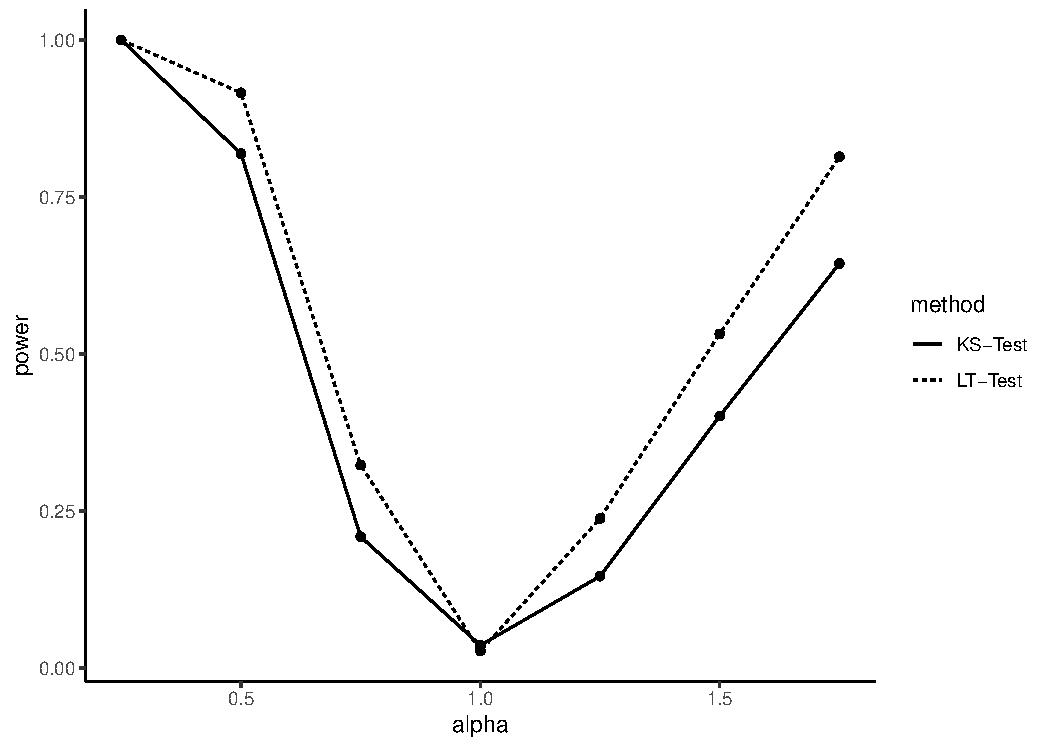
\includegraphics[width = 0.7\textwidth]{../figures/power_LT_VS_KS}
\caption{Puissance du LT test et du test de K-S.}
\label{fig:power_LT_VS_KS}
\end{figure}
\part Commenter le résulat de la Figure \ref{fig:power_LT_VS_KS}.
\begin{itemize}
 \item La forme de la courbe est elle celle attendue? 
 \item Quel est le meilleur test?
\end{itemize}
Pour plus d'information sur ce test, on pourra se référer au travail de Henze et Meintanis \cite{Henze2002}
\begin{solution}
\begin{itemize}
	\item La forme de la courbe est celle attendue, pour $\alpha = 1$ les données provienne du modèle exponentielle, la puissance des test doit donc atteindre le niveau fixé à $0.05$ et augmenté de part et d'autre de $\alpha = 1$
	\item Le LT test semble supérieur. Il est tout à fait possible qu'un résultat inverse soit obtenu si les données proviennent d'un modèle de Weibull par exemple. On peut conclure que le LT test semble meilleur pour discriminer des données qui proviennent de la loi gamma.
\end{itemize}
\end{solution}
\end{parts}

\end{questions}
\bibliography{mdd.bib}
\bibliographystyle{plain}
\end{document}
